\chapter{Lec 16 - Bayesian Networks}
\section{Bayesian Networks}
This section introduces a data structure called a \textbf{Bayesian network} to represent the dependencies among variables. Bayesian networks can represent essentially
any full joint probability distribution and in many cases can do so very concisely.\\\\
A Bayesian network is a directed graph in which each node is annotated with quantitative probability information. The full specification is as follows:
\begin{itemize}
    \item  Each node corresponds to a random variable, which may be discrete or continuous.

    \item A set of directed links or arrows connects pairs of nodes. If there is an arrow from node $X$ to node $Y$ , $X$ is said to be a parent of $Y$. The graph has no directed cycles (and hence is a directed acyclic graph, or DAG).

    \item  Each node $X_i$ has a conditional probability distribution $\textbf{P}(X_i | Parents(X_i)) $that quantifies the effect of the parents on the node.
\end{itemize}
The topology of the network, the set of nodes and links, specifies the conditional independence relationships that hold in the domain. In the simplest case, each conditional distribution is represented as a \textbf{conditional probability table} (\textbf{CPT}) giving the distribution over $X_i$ for each combination of parent values.\\\\
Now consider the following example.  You have a new burglar alarm installed at home. It is fairly reliable at detecting a burglary, but also responds on occasion to minor earthquakes. You also have two neighbors, John and Mary, who have promised to call you at work when they hear the alarm. John nearly always calls when he hears the alarm, but sometimes confuses the telephone ringing with the alarm and calls then, too. Mary, on the other hand, likes rather loud music and often misses the alarm altogether. Given the evidence of who has or has not called, we would like to estimate the probability of a burglary.
\begin{center}
    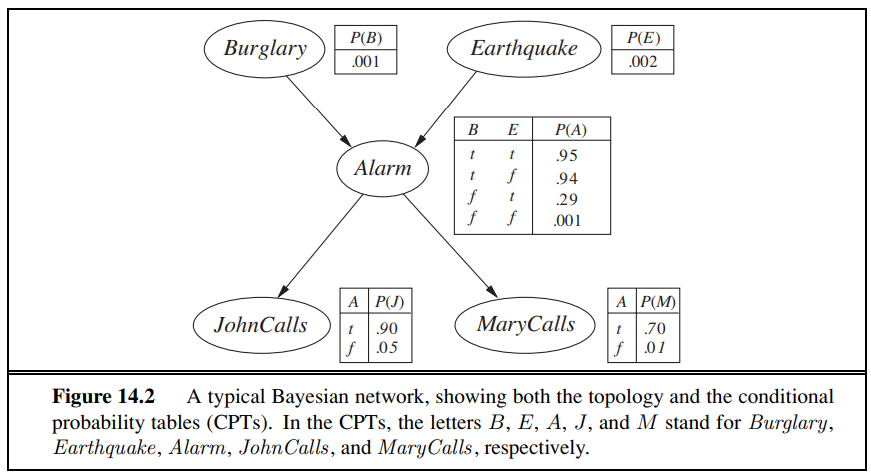
\includegraphics[scale=0.9]{images/bayes-net-ex.png}
\end{center}
The figure above shows a Bayesian network for this domain.  Each row of a CPT must sum to 1, because the entries represent an exhaustive set of cases for the variable. For Boolean variables, once you know that the probability of a true value is $p$, the probability of false must be $1 - p$, so we often omit the second number, as we do in the figure above.  In general, a table for a Boolean variable with $k$ Boolean parents contains $2^k$ independently specifiable probabilities. A node with no parents has only one row, representing the prior probabilities of each possible value of the variable. If a variable $X$ can take $m$ different values, the number of parameters required to represent a distribution over $X$ is given by:
\[(m-1)\prod_{xp \in Parent(X)} m_{xp}\]
where $m_{xp}$ is the number of values that the parent $xp$ of $X$ can take.\\\\
To store the values of a complete network over $n$ Boolean variables we require $O(n \cdot 2^k)$ numbers. If we are able to find a good factorization of the full joint probability distribution exploiting conditional independence (i.e. keeping $k$ small), the number of required parameters grows linearly with $n$.

\section{Global semantics}
The previous section described what a network is, but not what it means. There are two ways in which one can understand the semantics of Bayesian networks. The first is to see the network as a representation of the joint probability distribution. The second is to view it as an encoding of a collection of conditional independence statements.\\\\
One way to define what the network means is to define the way in which it represents a specific joint distribution over all the variables.\\\\
A generic entry in the joint distribution is the probability of a conjunction of particular assignments to each variable, such as $P(X_1 = x_1 \land ... \land X_n = x_n)$. We use the notation $P(x_1,...,x_n)$ as an abbreviation for this. The value of this entry is given by the formula:
\[P(x_1, ..., x_n) = \prod_{i=1}^n P(x_i | parents(X_i))\]
where $parents(X_i)$ denotes the values of $Parents(X_i)$ that appear in $x_1,...,x_n$. Basically, it defines the full joint distribution as the product of the local conditional distributions.\\\\
To illustrate this, we can calculate the probability that the alarm has sounded, but neither a burglary nor an earthquake has occurred, and both John and Mary call. We multiply entries from the joint distribution (using single-letter names for the variables):
\[\begin{split}
    P(j, m, a,\neg b,\neg e) & = P(j | a)P(m | a)P(a | \neg b \land \neg e)P(\neg b)P(\neg e)\\
    & = 0.90 \times 0.70 \times 0.001 \times 0.999 \times 0.998 = 0.000628 .
\end{split}\]
If a Bayesian network is a representation of the joint distribution, then it too can be used to answer any query, by summing all the relevant joint entries as we saw previously.

\section{Complexity of exact inference}
In the previous chapters we saw that any conditional probability can be computed by summing terms from the full joint distribution.  More specifically, a query $\textbf{P}(X | \textbf{e})$ can be answered using
\[\textbf{P}(X | \textbf{e}) = \alpha \textbf{P}(X, \textbf{e}) = \alpha \sum_{\textbf{y}}\textbf{P}(X, \textbf{e}, \textbf{y})\]
Now, a Bayesian network gives a complete representation of the full joint distribution. More specifically, we have seen that the joint distribution can be written as products of conditional probabilities from the network. Therefore, a
query can be answered using a Bayesian network by computing sums of products of conditional probabilities from the network.\\\\
Consider the query $\textbf{P}(Burglary | JohnCalls = true, MaryCalls = true)$. The hidden variables for this query are $Earthquake$ and $Alarm$. Then, we have:
\[\textbf{P}(B | j, m) = \alpha \textbf{P}(B, j, m) = \alpha \sum_e \sum_a \textbf{P}(B, j, m, e, a)\]
The semantics of Bayesian networks then gives us an expression in terms of CPT entries. For simplicity, we do this just for $Burglary = true$:
\begin{equation}
    P(b | j, m) = \alpha \sum_e \sum_a P(b)P(e)P(a|b, e)P(j|a)P(m|a)
\end{equation}
The complexity of exact inference in Bayesian networks depends strongly on the structure of the network. The burglary network we presented previously belongs to the family of networks in which there is at most one undirected path between any two nodes in the network. These are called \textbf{singly connected} networks or \textbf{polytrees}, and they have a particularly nice property: The time and space complexity of exact inference in polytrees is linear in the size of the network. Here, the size is defined as the number of CPT entries; if the number of parents of each node is bounded by a constant $k$, then the complexity will also be linear in the number of nodes, i.e., $O(n \cdot 2^k)$ for Boolean variables. Note that the complexity of an algorithm for computing Equation (1) is $O(n \cdot 2^n)$, but there are techniques that can speed up the computation which we won't see.
\\\\
For \textbf{multiply connected} networks exact inference can have exponential time and space complexity in the worst case, even when the number of parents per node is bounded (NP-Hard problem).


\section{Inference by stochastic simulation}
Given the intractability of exact inference in large, multiply connected networks, it is essential to consider approximate inference methods. The basic idea is to draw $N$ samples from a sampling distribution $S$ and compute an approximate posterior probability $\hat{\textbf{P}}$. Then, we expect $\hat{\textbf{P}}$ and the true probability $\textbf{P}$ to converge as $N$ increases. There exist severs approaches:
\begin{itemize}
    \item \textbf{Direct sampling:}  The idea is to sample each variable in turn, in topological order.

    \item \textbf{Rejection sampling} 

    \item \textbf{Likelihood weighting}

    \item \textbf{Markov chain Monte Carlo (MCMC)}
\end{itemize}
